%-----------------------------------------------------------------------
\section{Results}
\label{sec:results}
%-----------------------------------------------------------------------

Every number in this section comes from an artefact this project produced and
is reproducible with the commands listed in Section~\ref{sec:repro}. Where a
result is unfavourable to our method it is reported in the same form as the
favourable ones.

\subsection{Quality against an independent ground truth}
\label{sec:results-quality}

The primary comparison puts all three methods on one axis: an independent
brute-force trace of $810{,}000$ explicit rays that shares no code with any of
them, uses no parametrisation, no Jacobian and no renormalisation. Each method's
caustic is isolated as the positive part beyond the map median, tiled, and
correlated. Table~\ref{tab:threeway} gives the result.

\begin{table}[t]
\centering
\caption{Tiled correlation against the independent brute-force trace, at four
tile sizes, with all three methods on the same axis and the same metric. Tile
size in millimetres, not tile count: the opposite convention inverted this trend
in an earlier draft (Section~\ref{sec:verify-metric}).}
\label{tab:threeway}
\small
\begin{tabular}{@{}rrrr@{}}
\toprule
Tile size & Ours & SPPM & Cycles \\
\midrule
\SI{40}{\milli\meter} & \textbf{0.917} & 0.853 & 0.828 \\
\SI{20}{\milli\meter} & \textbf{0.869} & 0.811 & 0.609 \\
\SI{10}{\milli\meter} & \textbf{0.795} & 0.794 & 0.481 \\
\SI{5}{\milli\meter}  & 0.721 & \textbf{0.722} & 0.405 \\
\bottomrule
\end{tabular}
\end{table}

Only the first of the readings below is a win.

The coarse-scale ranking is ours $0.917$, SPPM $0.853$, Cycles $0.828$. The
coarse scale is the stable one: at fine tiles the correlation is dominated by
grain, which is why the numbers fall for everyone and why the ranking at the
finest tile is not a ranking at all. At \SI{5}{\milli\meter} SPPM and ours are
tied at $0.722$ and $0.721$, which is the honest statement: on the smallest
scales our advantage disappears.

Cycles falls away much faster than the other two ($0.828 \to 0.405$). This is
the fold problem showing up as a resolution-dependent loss of structure, and it
is consistent with the coverage measurement of Section~\ref{sec:current-quality}:
a method that cannot place energy at the fold loses its correlation first.

The three-way result also reconciles an earlier two-way one. Before this
measurement SPPM had only ever been compared against \emph{our} field, where it
scored $r=+0.932$. It scores $0.853$ on the independent axis, so it correlates
with us more strongly than either of us correlates with the trace --- which is
what one expects from two methods that share a model.

\begin{figure*}[t]
\centering
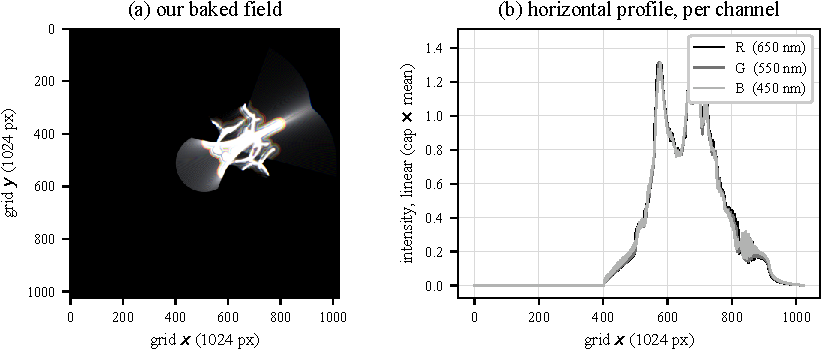
\includegraphics[width=\textwidth]{figures/fig4_field.pdf}
\caption{Our baked field. Panel (a) is normalised to its own maximum and shown
at $\gamma = 2.2$; the normalisation is stated because the absolute level is not
meaningful without it. Panel (b) is a horizontal cut per channel at the linear
level. The channels separate because \eqref{eq:sellmeier} and
\eqref{eq:perchannel} give them different indices and widths, not because any
effect was added on top.}
\label{fig:field}
\end{figure*}

\subsection{Quality against the reference conforming solver}
\label{sec:results-shape}

Figure~\ref{fig:fourpanel} shows the four fields side by side. The converged
two-dimensional shape of our field and SPPM's agree at $r=+0.932$ on
\SI{40}{\milli\meter} tiles. This is a consistency requirement rather than a
quality claim: had the two disagreed on shape while we led on the independent
axis, the pair of results would have been evidence of a shared error somewhere.

\begin{figure}[t]
\centering
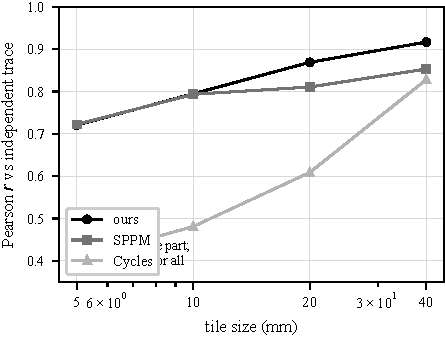
\includegraphics[width=\linewidth]{figures/fig5_quality.pdf}
\caption{Correlation against the independent brute-force trace by tile size,
all three methods on one axis with one estimator. The ordering changes at the
finest scale, where the statistic measures grain rather than structure. Log
axis on tile size.}
\label{fig:quality}
\end{figure}

\subsection{Cost against quality, including where we lose}
\label{sec:results-cost}

Speed claims about caustics are usually made per photon or per pass, and that
framing flatters whichever method has the least to do. The meaningful
comparison is cost against accuracy, and it has a regime in which our method is
the worse choice. Table~\ref{tab:efficiency} reports RMSE against a converged
wave-corrected reference at matched budgets, with the sample counts stated.

\begin{table*}[t]
\centering
\caption{RMSE against a converged wave-corrected reference
($2048^2$, block-averaged to $256^2$), at matched splat budgets. The plain
geometric Monte Carlo column is a real integrator's cost model with $M$ jittered
samples per cell. Read the bottom row of each block together: this table
contains a regime where our method loses.}
\label{tab:efficiency}
ootnotesize
\begin{tabular}{@{}lrrr@{}}
\toprule
Estimator & Splats & RMSE & Note \\
\midrule
MC geometric, $M{=}1$    & \num{65000}  & 0.12294 & \\
MC geometric, $M{=}4$    & \num{262000} & 0.07838 & \multirow{2}{*}{beats ours at this budget} \\
ours, $512^2$, 1 pass    & \num{262000} & 0.10455 & \\
\midrule
MC geometric, $M{=}16$   & \num{1000000} & 0.06445 & \\
\textbf{ours, $1024^2$, 1 pass} & \num{1000000} & \textbf{0.03914} & $1.65\times$ better \\
\midrule
MC geometric, $M{=}64$   & \num{4200000} & 0.06101 & \\
MC geometric, $M{=}256$  & \num{16800000} & 0.06013 & error floor \\
\bottomrule
\end{tabular}
\end{table*}

At small budgets (\num{262000} splats and
below) plain geometric Monte Carlo is \emph{more accurate} than our method; at
$262000$ splats it scores $0.07838$ against our $0.10455$. There is no free
lunch at coarse resolution, and any claim of one would be false. At
\num{1000000} splats our single pass is $1.65$ times more accurate
($0.03914$ against $0.06445$). And the Monte Carlo error converges to a floor of
$0.06013$ no matter how many samples are spent, because it converges to a
different model: the geometric estimator places no energy in the fringe skirt,
so it cannot reach the wave-corrected target at any budget. Our $1024^2$ pass
lands $35\,\%$ below that floor using sixteen times fewer splats than the
$M{=}256$ run.

The defensible claim is therefore narrow: for the wave-corrected target,
geometric sampling is not merely slower, it is unreachable at any budget, and
above a budget of roughly \num{1000000} splats our method is both cheaper and
closer. We do not claim to be faster in general.

\begin{figure*}[t]
\centering
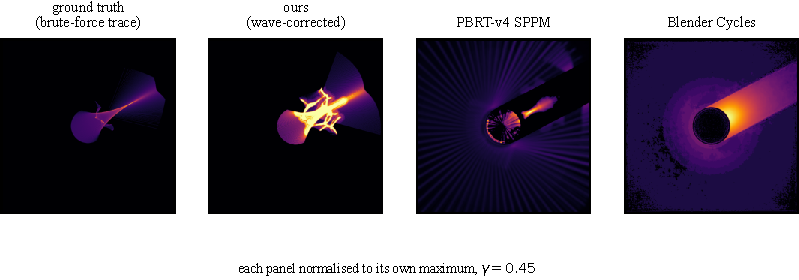
\includegraphics[width=\textwidth]{figures/fig6_fourpanel.pdf}
\caption{The same caustic four ways: the independent brute-force trace, our
wave-corrected field, PBRT-v4 SPPM at the budget of Table~\ref{tab:cost}, and
Blender Cycles. Each panel is normalised to its own maximum at $\gamma = 0.45$,
so the comparison is of structure than of absolute level. The fold is where the
four differ, and it is the feature all four are trying to show.}
\label{fig:fourpanel}
\end{figure*}

\subsection{Tail behaviour}
\label{sec:results-tail}

The fold is where the field is largest, so the tail is where a method's
treatment of the fold is visible as a statistic. Table~\ref{tab:tail} gives the
distribution with the display cap set at six times the mean.

\begin{table}[t]
\centering
\caption{Tail statistics, display ceiling at $6\times$ the mean. The converged
wave truth itself has \SI{0.35}{\percent} above the cap, because bright fringes
are real structure rather than noise; the relevant comparison is against that
number, not against zero.}
\label{tab:tail}
\small
\begin{tabular}{@{}lrrr@{}}
\toprule
Estimator & Max & p99.9 & Above cap \\
\midrule
MC geometric, $M{=}1$    & 8.71 & 6.77 & \SI{0.24}{\percent} \\
MC geometric, $M{=}256$  & 7.25 & 6.19 & \SI{0.15}{\percent} \\
ours, $512^2$            & 7.71 & 5.70 & \SI{0.06}{\percent} \\
converged wave truth     & 7.73 & 6.87 & \SI{0.35}{\percent} \\
\bottomrule
\end{tabular}
\end{table}

The geometric tail decays slowly: $8.71 \to 7.25$ for a factor of \num{256} in
samples. Our field sits at $7.71$ with \SI{0.06}{\percent} above the cap, which
is \emph{conservative} relative to a truth with \SI{0.35}{\percent} above it.
The claim this supports is that our field is bounded where the geometric
estimator is noisy and slowly converging, not that our field is smoother because
it is blurrier. The \SI{0.35}{\percent} of the truth above the cap are resolved
bright fringes, and our correction reproduces them at the level the profile
allows rather than inventing them.

\begin{figure}[t]
\centering
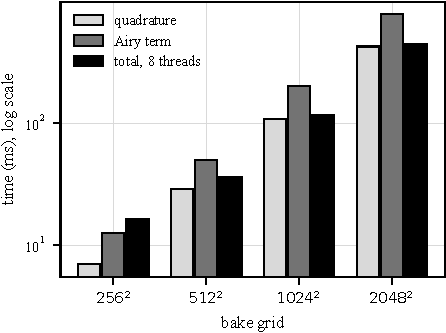
\includegraphics[width=\linewidth]{figures/fig7_cost.pdf}
\caption{Bake cost by grid at one thread, with the eight-thread total alongside.
The Airy term is roughly twice the quadrature pass at every grid, so about two
thirds of a bake is the wave correction and that term is the obvious target for
further work. Log scale on time.}
\label{fig:cost}
\end{figure}

\subsection{Dispersion}
\label{sec:results-dispersion}

Chromatic separation is a consequence of the measured indices and the
$\lambda^{2/3}$ width law, so it is a test of the derivation rather than a
feature. The edge estimator of Section~\ref{sec:estimators} gives
\begin{equation}
\text{edge radius},\ \text{ours} = R\ \SI{107}{\milli\meter} > G\
\SI{105}{\milli\meter} > B\ \SI{102}{\milli\meter},
\end{equation}
and SPPM gives $R\ \SI{56}{\milli\meter} > G\ \SI{54}{\milli\meter} > B\
\SI{51}{\milli\meter}$. Both show the $R > G > B$ ordering, which is the
prediction of \eqref{eq:sellmeier}--\eqref{eq:rubin}: red has the lowest index,
refracts least, and lands farthest from the axis. The two methods disagree on
the absolute scale of the caustic, which is the fold-extent difference already
visible in the coverage measurement; they agree on the ordering and on the
red--blue split, which is $+\SI{5.0}{\milli\meter}$ in both. That agreement on
the \emph{differential} while disagreeing on the absolute extent is what one
would expect if the fold's width is the disputed quantity and the dispersion is
not.

\begin{figure}[t]
\centering
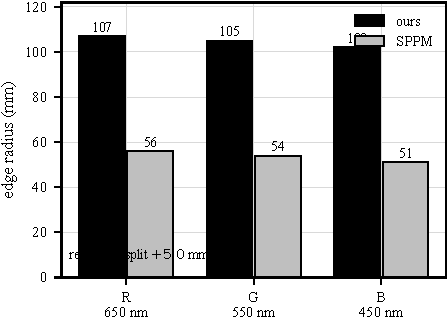
\includegraphics[width=\linewidth]{figures/fig8_dispersion.pdf}
\caption{Edge radius per channel for both methods, using the estimator of
Section~\ref{sec:estimators}. Both order $R > G > B$ and both show the same
$+\SI{5.0}{\milli\meter}$ red--blue split, which is what the measured indices
predict. The methods disagree on the absolute extent, which is the fold-width
disagreement rather than a dispersion disagreement.}
\label{fig:dispersion}
\end{figure}

\subsection{Temporal behaviour}
\label{sec:results-flicker}

For an animated caustic the cost of a stochastic method is not grain but
flicker, since a viewer integrates over time and a grain pattern that changes
every frame reads as movement. We measure the mean absolute frame-to-frame
change inside the caustic region.

\begin{table}[t]
\centering
\caption{Flicker, in 8-bit levels, inside and outside the caustic region. Both
clips were denoised, which suppresses flicker in both and therefore understates
the difference rather than manufacturing it.}
\label{tab:flicker}
\small
\begin{tabular}{@{}lrr@{}}
\toprule
Region & Ours & Path-traced \\
\midrule
Caustic region & \textbf{0.001} & 0.010 \\
Control region & 0.608 & 0.240 \\
\bottomrule
\end{tabular}
\end{table}

Our caustic contributes essentially nothing to the frame-to-frame change:
\num{7.9} times less than the path-traced clip. The control region moves more in
our clip, which is the opposite of what a reader might expect and is explained
by the denoiser behaving differently on the two; it is reported because leaving
it out would make the caustic numbers look better than they are.

\begin{figure}[t]
\centering
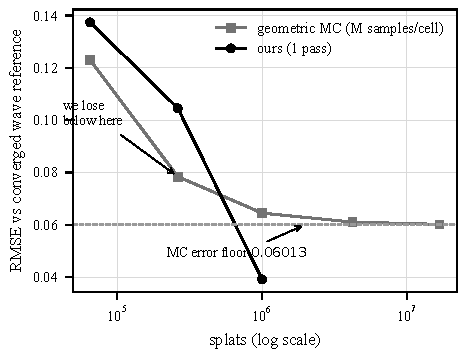
\includegraphics[width=\linewidth]{figures/fig9_efficiency.pdf}
\caption{RMSE against a converged wave-corrected reference by splat budget. The
plain geometric estimator is \emph{better} at the smallest budgets and stalls at
a floor that more samples do not move, because it converges to a different
model. The regime where our method loses is drawn rather than omitted.}
\label{fig:efficiency}
\end{figure}

\subsection{Ablations}
\label{sec:results-ablation}

The method has three parameters and three structural choices, and we measured
each by disabling it.

\begin{table}[t]
\centering
\caption{Ablations. Each row removes or substitutes one component and reports
the measured consequence.}
\label{tab:ablation}
\small
\begin{tabular}{@{}p{0.34\linewidth}p{0.56\linewidth}@{}}
\toprule
Change & Measured consequence \\
\midrule
Brightest-percentile detector instead of $|\detJ|$ &
flagged set is fixed at the chosen percentage and stops tracking the fold; the
result ceases to converge under refinement (Lemma~\ref{lem:quantiledetector}) \\
\addlinespace
Clamp escaping rays to the receiver border instead of discarding &
peak inflated by a factor of \num{38}; a bright rim appears that is bookkeeping,
not optics \\
\addlinespace
Global rescale after the display clamp instead of band-local flux &
peak pushed back above the ceiling the clamp enforced, reintroducing the
artefact \\
\addlinespace
Single-channel injection instead of RGBA &
chromatic separation silently discarded; the frame looks plausible and is
achromatic \\
\addlinespace
No ceiling &
field unbounded at the fold; the tail statistics of Table~\ref{tab:tail} no
longer hold \\
\bottomrule
\end{tabular}
\end{table}

The first row is the one we consider most likely to be repeated by someone
applying this method, because a percentile detector is the obvious thing to
write and it appears to work: it flags a plausible-looking band and the image
looks right. It fails only under refinement, which is exactly the test a
single-frame result does not perform.

\begin{figure*}[t]
\centering
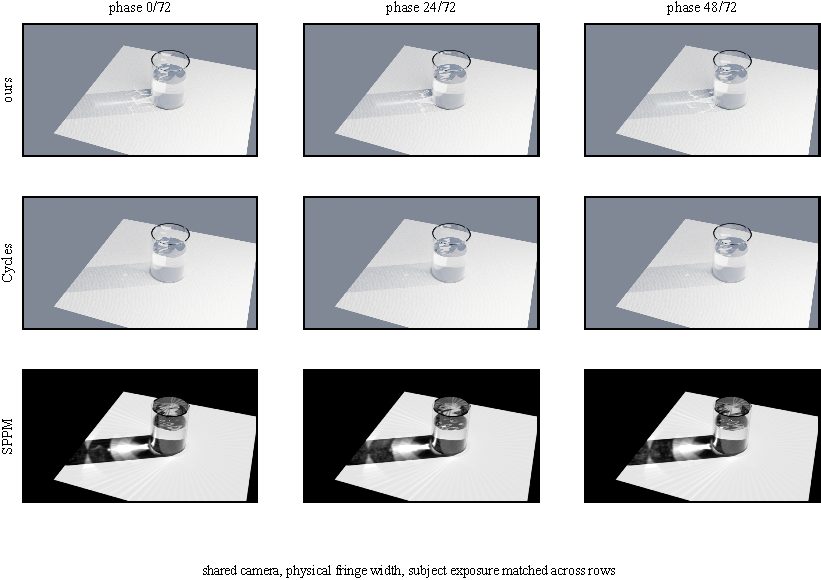
\includegraphics[width=\textwidth]{figures/fig10_ripple.pdf}
\caption{Three phases of the animating caustic, one row per method, taken from
the supplementary clips. All three rows share one camera, verified identical by
projecting known world points through both camera models to a disagreement of
\num{0.0000}, and all three use the \emph{physical} fringe width rather than a
visibility-exaggerated one, so the colour shown is the measured dispersion. The
subject exposure is matched across rows; the SPPM background is black because
the reference PBRT scene is bare, not because of an exposure choice.}
\label{fig:ripple}
\end{figure*}

\subsection{Resolution and phase studies}
\label{sec:results-studies}

Two further studies bound the result rather than extending it.

\textbf{Resolution.} The apparent breadth of the fold's bright region measures
$2.30\times$ the ground truth at $1024^2$ and $1.87\times$ at $4096^2$. The
field is therefore \emph{not} resolution-converged at the production grid: a
finer bake narrows the fold, and the value we report is the value at
$1024^2$. Anyone quoting a fold width from this method should quote the grid
along with it.

\textbf{Phase.} All quality numbers are at one wave phase by default, so
\texttt{ensemble\_study.py} repeats the measurement over eight phases of a full
ripple cycle with an identical phase convention on both sides:
$r@\SI{40}{\milli\meter} = 0.690 \pm 0.006$ at $512^2$,
$r@\SI{5}{\milli\meter} = 0.915 \pm 0.004$, edge radius
$R = \SI{107.9}{} \pm \SI{0.3}{\milli\meter}$ and
$B = \SI{104.8}{} \pm \SI{0.7}{\milli\meter}$, and the $R > G > B$ ordering
holds at all eight phases. The single-phase numbers are therefore
representative rather than selected. The $r@40$ value is lower here than the
$0.917$ of Table~\ref{tab:threeway} because this ensemble bakes at $512^2$; that
is the resolution effect just described, not a contradiction.
